\documentclass{article}
\usepackage{fullpage}
\usepackage{graphicx}

\title{CHREST Manual \\ (version 4.0.0)}
\author{Peter Lane}

\begin{document}
\maketitle

\begin{abstract}

\noindent CHREST is a symbolic cognitive architecture explaining how experience
affects our ability to remember, categorise and think about the world.  This
document contains a technical description of CHREST, including details of its
operation and links to the implementation.  A separate user guide is available,
which is a gentler introduction to using the CHREST software.

\end{abstract}

\tableofcontents
\newpage

\section{Overview of CHREST Architecture}

The CHREST architecture may be broadly divided into four components.
Interactions with the world pass through an input/output component, which is
responsible for interpreting inputs as patterns and for converting action
patterns into operations on the world.  Patterns are passed through the
chunking network, which acts as an index into long-term memory.  Chunks
retrieved from long-term memory are placed into the short-term (or working)
memory, which is a limited capacity store.  Figure~\ref{chrest-architecture}
provides an overview of these components and their connections.

\begin{figure}
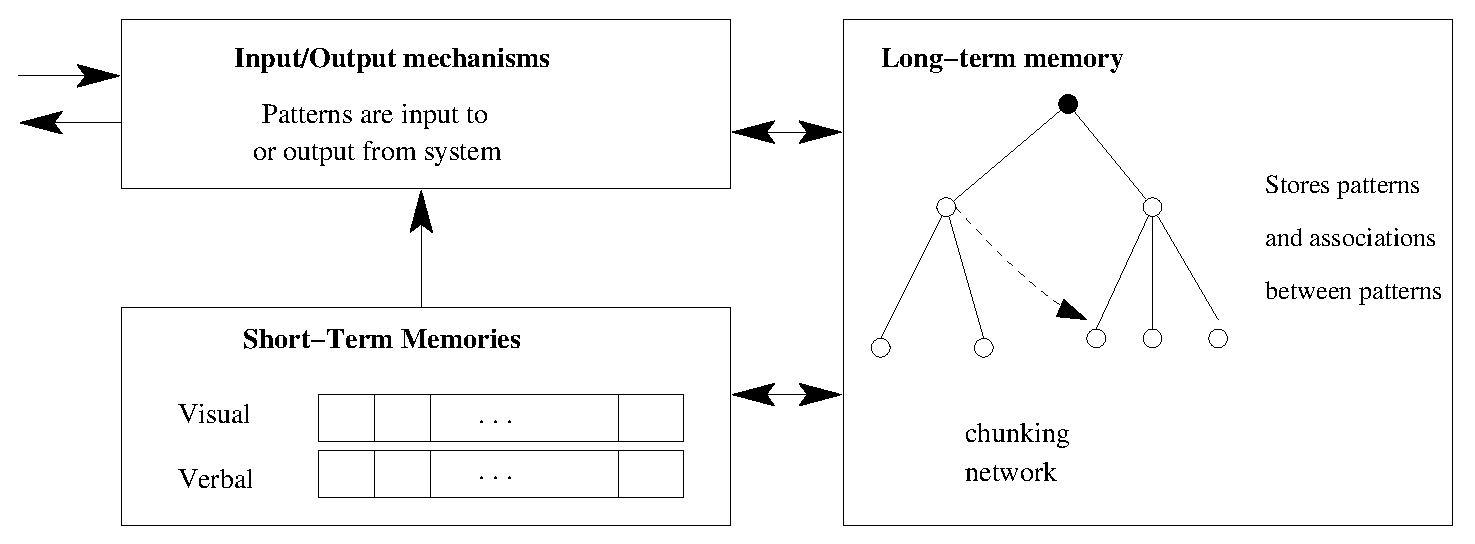
\includegraphics[width=\textwidth]{figures/chrest.eps}
\caption{An overview of CHREST}
\label{chrest-architecture}
\end{figure}

The distinctive aspect and role of CHREST is in accessing appropriate long-term
memory structures given a perceived stimulus, such as an image or spoken
sentence.  The architecture explains how memories are accessed given some
input, and how certain kinds of associations can be constructed across elements
of declarative or procedural memory when primed by perception.  The {\em
chunking network} provides the index into long-term memory, and is constructed
in close association with the perceptual mechanisms, which control eye
movements or how verbal information is stored for rehearsal.

CHREST thus has links to the following kinds of memories, but does not provide
a fully-worked out theory of them:

\begin{itemize}
\item Procedural memory: unconscious memory of skills
\item Declarative memory: conscious memory of facts
\begin{itemize}
\item Episodic memory: facts about one's own life
\item Semantic memory: facts about the world and their connections
\end{itemize}
\end{itemize}

With only a small emphasis on procedural and declarative memory, CHREST has a
different focus than architectures such as Soar~\cite{Laird12,Newell90} or
ACT-R~\cite{Anderson98}.  However, with a greater emphasis on learning and the 
link between learning and perception, CHREST provides an explanation of how 
experience affects our ability to remember, categorise and think about the 
world around us.

This document describes in more detail each component of CHREST.  We begin with
the long-term memory structures: the chunking network, the semantic memory and
templates.  Then we cover the perception module, based on Perceiver, and the
short-term or working memory, followed by explaining the mechanisms for
including emotional responses in learning and retrieval.  We bring these
components together by explaining how to control and work with a CHREST-based
agent.  Finally, we introduce some example domains and models.

\section{Chunking Network}


\section{Semantic Memory and Templates}

\subsection{Semantic Links}

In EPAM, Simon's model of Memory from which CHREST is inspired, nodes are
connected by tests used in the discrimination process.  Although nodes are also
supposed to be connected by semantic links, a common idea in cognitive
psychology, this is not implemented in EPAM.  CHREST~2 introduced the idea of
semantic links, to make the model a more plausible theory of human memory.

The basic idea is that nodes that have a similar internal representation (in the case
of CHREST, patterns of chess pieces) are connected together by links. 

\subsubsection{How are semantic links created?}

Chunks stored in STM are compared pairwise, and if their images 
(internal representation) overlap with at least the minimum of elements set
by the {\tt similarity threshold} parameter, a link is created.

Example:

Assume that pointers to Node-1 and Node-2 are stored in STM. The images of the
nodes are as follows:

\begin{verbatim}
node-1-image:  ("Pc4" "Pd5" "Pe4" "Pf3" "Nc3" "Be3")
node-2-image:  ("Pd5" "Pe4" "Nc3" "Be3")
\end{verbatim}

assume also that the {\tt similarity threshold} is set to 4.

In this case, 4 pieces-on-squares are members of both images, so the criterion 
is met, and a semantic link is created. A pointer to node-1 is added to 
the list of semantic links for node-2, and a pointer to node-2 is added to 
the list of semantic links for node-1.

\subsubsection{How are semantic links used during pattern recognition?}

When recognising a pattern, the program uses the discrimination net as before.
The difference is that when a leaf node is reached, this node is not returned
immediately, but the program searches through the nodes connected by semantic
links to see if some node has richer information, as calculated by the size of
the image and the number of slots in the template (see below). The depth of
search is controlled by the parameter {\tt maximum semantic distance}. This
parameter is set to 1 currently: only nodes one semantic link away from the
node reached by discrimination can be selected.  (This parameter is not
accessible in the GUI.)

The effect of the semantic links is to make all search paths to one of the
nodes in the semantic network always reach the most informative
semantically-equivalent node.  As these connections and relations are computed
based on the current state of the network, subsequent learning in other parts 
of the network may alter the node retrieved for any given input pattern.

\subsection{Templates}

The idea of templates is discussed in detail in~\cite{Gobet96b}.  The basic
idea is that some chunks, which occur often when playing or studying games,
evolve into more complex data structures, which possess slots supporting the
storage of variable information.  Templates are also supposed to point to other
types of information: moves, plans, evaluation of the position described in the
template, and so on, but this has not been implemented yet.

\subsubsection{How templates are created}

Slots are created for types of information that recur often. There are two
sources for the information: nodes reached via test links, and nodes reached
via semantic links.  For the nodes located at a minimum-level in the network,
CHREST looks for if some information (type of piece, square or chunk) recurs at
least a minimum-number-of-occurrences. If this is the case, a slot is created
for this type of piece, square or chunk.\footnote{Note: slots for chunks are
not currently implemented.}

Note that in the present version, templates are created periodically during 
the learning phase: the whole net is scanned and templates are created when 
possible. This is done mainly for efficiency and simplicity reasons. 
Later versions will probably have nodes checked for templates when they are 
recognized during the learning phase.

\subsubsection{How templates are used during a memory task}

During the presentation of a position, the program recognizes patterns of
pieces on squares, and outputs a node. If the node is a template, the program
tries to fill in slots of this template with pieces on squares in the pattern
that do not belong to the image of the node. In addition, the program tries to
fill in slots of the hypothesis with each pattern newly perceived. During the
reconstruction phase, information in slots is used as any other information
stored in STM.

In the current version, slots may be filled in with any type of information
that shares the piece, square or chunk labeling the slot. A possibly more
plausible mechanism is that slots may be rapidly instantiated only with
information already present in the net.  With method (a) of construction, for
example, slots could be filled in only with values that appear in at least one
of the links coming from the template-node.


\section{Perceiver}

The Perceiver is responsible for gathering information from a visual stimulus.
Input from the simulated eye is in the form of {\em patterns}, containing 
a sequence of {\em item-on-square}.

Attention is controlled using a set of heuristics.  In line with studies 
on expertise, the heuristics vary slightly between novice and experts.  An 
arbitrary dividing line is placed between novice and experts at 2000~nodes in 
visual LTM.

The heuristics are as follows:

\paragraph {LTM}

\paragraph {Neighbouring piece}

The heuristics are applied, as shown in Table~\ref{heuristics}.

\begin{table}
\begin{tabular}{cc}
A & B\\
\end{tabular}
\caption{Heuristics}
\label{heuristics}
\end{table}


\section{Working Memory}

\section{Emotions}

\section{Controlling a Model}

\section{Examples}

The following examples demonstrate the use of CHREST in three domains taken
from published work.  More examples are provided in the `examples' folder of
the distributed software.

\subsection{Chess recall}

Based on book~\cite{deGroot96} and article~\cite{Gobet00b}.

\subsection{Language learning}

Based on EPAM-VOC~\cite{Jones08}.

\subsection{Iowa gambling task}

Based on Marvin's project~\cite{Gobet11a}.

\section{Recommended reading}

The following publications are recommended for understanding the current 
status of CHREST and related models.

\begin{itemize}
\item A general description of chunking mechanisms in human learning.\cite{Gobet01}
\end{itemize}


\subsection{Historical background}

The following publications may be of interest for understanding the development 
of CHREST and its precursors.

\subsubsection{CHREST and related models}

{\em Version~1 of CHREST} was released in 1993 and published as:

\begin{itemize}
\item F. Gobet (1993). Les memoires d'un joueur d'\'echecs.~\cite{Gobet93a}
\item F. Gobet (1993). A computer model of chess memory.~\cite{Gobet93b}
\end{itemize}

A variant of the first version of CHREST was described in chapter~8 of~\cite{deGroot96}.
The main differences in comparison with the first version were that the
internal representation does not play any more the role of a retrieval
structure, and that the eye movements were simulated much more closely than in
the earlier version. 
\vspace{3pt}

\noindent {\em Version~2 of CHREST} was released in 1995 and included the
ideas of semantic links between nodes and templates.  Important publications
for version~2 include:

\begin{itemize}
\item F. Gobet and H.A. Simon (1996), Templates in chess memory: A mechanism for 
recalling several boards.~\cite{Gobet96b}
\item F. Gobet, Memory for the meaningless: How chunks help.~\cite{Gobet98a}
\end{itemize}

\noindent {\em CHUMP} is a version of CHREST which learns to select moves by pure
pattern recognition (no search):

\begin{itemize}
\item F. Gobet \& P. Jansen (1994). Towards a chess program based on a model of
human memory.~\cite{Gobet94} 
\end{itemize}

\noindent {\em Version~3 of CHREST} was released in 2009, and used in modelling
some further results in chess expertise, particularly short-term memory
effects.

\begin{itemize}
\item R. Ll. Smith, F. Gobet and P.C.R. Lane (2007), An investigation into the
effect of ageing on expert memory with CHREST.~\cite{Smith07}
\item R. Ll. Smith, P.C.R. Lane and F. Gobet (2008), Modelling the relationship
between visual short-term memory capacity and recall ability.~\cite{Smith08}
\item R. Ll. Smith, F. Gobet and P.C.R. Lane (2009), Checking chess checks with
chunks: A model of simple check detection.~\cite{Smith09}
\end{itemize}

\noindent {\em Version~4 of CHREST} is due for release in late 2012, and is a
complete reimplementation of CHREST from Lisp into Java.  Version~4 includes
the components of earlier versions of CHREST, such as the chunking network,
semantic links, templates, perceiver and working memory, additionally supports
CHUMP~\cite{Bossomaier12,Gobet94}, and includes the emotion-handling
mechanisms, as developed by Marvin Schiller~\cite{Gobet11a}.

\subsubsection{Precursors of CHREST}

CHREST's chunking network is at heart a discrimination net similar (but not
identical) to that proposed by the EPAM theory.

\begin{itemize}
\item E.A. Feigenbaum \& H.A. Simon (1962). A theory of the serial position
effect.~\cite{Feigenbaum62}
\item E.A. Feigenbaum, \& H.A. Simon (1984). EPAM-like models of recognition 
and learning.~\cite{Feigenbaum84}
\item H.B. Richman \& H.A. Simon (1989). Context effects in letter
perception: Comparison of two theories.~\cite{Richman89}
\item H.B. Richman \& H.A. Simon (1994). EPAM simulations of short-term
memory.~\cite{Richman94} 
\item H.B. Richman, H.A. Simon \& F. Gobet (1991, July).
Applying retrieval structures to chess memory.~\cite{Richman91}
\item H.B. Richman, J. Staszewski \& H.A. Simon (1995). Simulation of expert memory with EPAM IV.~\cite{Richman95}
\end{itemize}

\noindent EPAM-based models have been used in chess:

\begin{itemize}
\item G.W. Baylor \& H.A. Simon (1966). A chess mating combinations program.~\cite{Baylor66}
\item H.A. Simon \& M. Barenfeld (1969). Information processing analysis of perceptual processes in problem solving.\cite{Simon69b}
\item H.A. Simon \& K.J. Gilmartin (1973). A simulation of memory for 
chess positions.~\cite{Simon73}
\end{itemize}




\bibliographystyle{plain}
\bibliography{/home/peter/Documents/biblio}

\end{document}

